\documentclass{beamer}

% Theme
\usetheme{Madrid}
\usecolortheme{default}

% Packages
\usepackage[utf8]{inputenc}
\usepackage[T1]{fontenc}
\usepackage{amsmath, amssymb, amsthm, dsfont}
\usepackage{graphicx}
\usepackage{tikz}
\usetikzlibrary{arrows.meta,positioning,calc}
\usepackage{caption}
\usepackage{hyperref}
\usepackage{centernot}

% Macros (standardized notation aligned with Lesson 1)
\newcommand{\R}{\mathbb{R}}
\renewcommand{\P}{\mathbb{P}}
\newcommand{\E}{\mathbb{E}}
\newcommand{\Var}{\operatorname{Var}}
\newcommand{\1}{\mathbf{1}}
\newcommand{\indep}{\perp\!\!\!\perp}
\newcommand{\toP}{\xrightarrow{\,\mathsf{P}\,}}
\newcommand{\toas}{\xrightarrow{\,\mathsf{a.s.}\,}}
\newcommand{\tod}{\xrightarrow{\,\mathcal{D}\,}}

% Helper for robust top-line commands (avoids fragile leading-backslash insertion issues)
\newcommand{\robustcmd}[1]{\csname #1\endcsname}

% Show a mini table of contents at the beginning of each section
\AtBeginSection[]{
  \begin{frame}{Outline}
    \robustcmd{tableofcontents}[currentsection,hideothersubsections]
  \end{frame}
}

% Title (robust invocation)
\robustcmd{title}[Applied Statistics]{Introduction to Basic Elements of Statistics}
\robustcmd{author}{Stéphane Rivaud}
\robustcmd{institute}{INRIA Saclay}
\robustcmd{date}{Septembre 12, 2024}

% Begin document
\begin{document}

% Title page
\begin{frame}
  \robustcmd{titlepage}
\end{frame}

% Outline
\begin{frame}{Outline}
  \robustcmd{tableofcontents}
\end{frame}

\section{Motivation}

\begin{frame}{What are Statistics ?}
  \vspace{0.8cm}
  Probability of a coin toss: Heads or Tail ?
  \[\P(\text{Head}) = 1 - \P(\text{Tail}) = \theta\]

  \vspace{0.8cm}
  Statistics: is the coin fair ?
  \[\P(\theta \mid \text{Set of coin tosses}) = \frac{1}{2} \quad \text{(?)}\]

  $\longrightarrow$ What can we deduce from partial observation of a phenomenon ?\\

  {
    \begin{center}
      Probabilities and Statistics are \textbf{dual mathematical frameworks}.
    \end{center}
  }

\end{frame}

\begin{frame}{Cox-Jaynes Theorem: Quantifying plausibility}
  Hypothesis on the method:
  \begin{itemize}
    \item \textbf{Coherence} $\rightarrow$ If a result can be derived in many ways, all derivation should yield the same result.
    \item \textbf{Continuity of the method} $\rightarrow$ Changing the value of a parameter should not change the computation method.
    \item \textbf{Universality} $\rightarrow$ The computation method should be general and not tied to a specific case.
  \end{itemize}
  \vspace{0.5cm}
  Hypothesis on the practitioner:
  \begin{itemize}
    \item \textbf{Unambiguous specifications} $\rightarrow$ a proposition can only be understood in a unique way.
    \item \textbf{No hidden information} $\rightarrow$ the algorithm is given all relevant information available.
  \end{itemize}

  \centering
  $\Longrightarrow$ \textbf{Isomorph} to \textbf{probability} theory
\end{frame}

\begin{frame}{Some key points}
  \begin{itemize}
    \item What is \textit{\textbf{Applied} Statistics} ?
    \item[]
    \item What are the kinds of \textbf{questions} we can answer with statistics ?
    \item[]
    \item What is the importance of \textbf{data} (vs statistical theory) ?
    \item[]
    \item Why is there so much \textbf{computer science} in statistics ?
    \item[]
    \item What is the difference between \textbf{Statistics} and \textbf{Machine Learning} ?
  \end{itemize}
\end{frame}

% Frame with 4 pictures
\begin{frame}{Example: Basics}
  \begin{columns}

    % Left column (Top and Bottom)
    \begin{column}{0.5\textwidth}
      % Top left picture
      \begin{figure}
        \centering
        \includegraphics[width=0.8\textwidth]{images/casino.jpg} % Replace with your first image path
      \end{figure}

      % Bottom left picture
      \begin{figure}
        \centering
        \includegraphics[width=0.8\textwidth]{images/chess.jpg} % Replace with your second image path
      \end{figure}
    \end{column}

    % Right column (Top and Bottom)
    \begin{column}{0.5\textwidth}
      % Top right picture
      \begin{figure}
        \centering
        \includegraphics[width=0.8\textwidth]{images/network.jpeg} % Replace with your third image path
      \end{figure}

      % Bottom right picture
      \begin{figure}
        \centering
        \includegraphics[width=0.8\textwidth]{images/game of go.jpg} % Replace with your fourth image path
      \end{figure}
    \end{column}

  \end{columns}
\end{frame}

\begin{frame}{Example: Medical Diagnosis}
  \begin{columns}

    % Left column
    \begin{column}{0.4\textwidth}
      \begin{figure}
        \centering
        \includegraphics[width=0.8\textwidth]{images/dr_house.pdf} % Replace with your first image path
      \end{figure}
    \end{column}

    % Right column
    \begin{column}{0.6\textwidth}
      \begin{figure}
        \centering
        \includegraphics[width=0.9\linewidth]{images/diagnosis.png}
        \caption{Bayesian network for differential diagnosis}
      \end{figure}
    \end{column}

  \end{columns}
\end{frame}

\begin{frame}{Physics}
  \begin{columns}

    % Left column
    \begin{column}{0.5\textwidth}
      \begin{figure}
        \centering
        \includegraphics[width=0.8\textwidth]{images/astronomy.jpg} % Replace with your first image path
      \end{figure}
    \end{column}

    % Right column
    \begin{column}{0.5\textwidth}
      \begin{figure}
        \centering
        \includegraphics[width=0.8\linewidth]{images/higgs_boson.jpg}
      \end{figure}
    \end{column}

  \end{columns}
\end{frame}

\begin{frame}{Advanced Example: Natural Language Processing}
  \begin{columns}

    % Left column
    \begin{column}{0.5\textwidth}
      \begin{figure}
        \centering
        \includegraphics[width=0.8\textwidth]{images/translation.pdf} % Replace with your first image path
        \caption{Automatic translation}
      \end{figure}
    \end{column}

    % Right column
    \begin{column}{0.5\textwidth}
      \begin{figure}
        \centering
        \includegraphics[width=0.8\linewidth]{images/spam_detection.png}
        \caption{Spam detection}
      \end{figure}
    \end{column}

  \end{columns}
\end{frame}

% Section 1: Probability on Sets
\section{Probability on Sets}

\begin{frame}{Events and Realization}
  Let $\Omega$ be the space of events.\\
  \begin{itemize}
    \item An event $A$ is a subset of $\Omega$.
    \item A realization of event $A$ is an element $x \in A$.
  \end{itemize}
  \vspace{0.5cm}
  Example:
  \begin{itemize}
    \item Dice rolls
    \item Next opponent move in Chess game.
    \item Result of a Chess game.
  \end{itemize}
\end{frame}

% Event Space, Events, and Realizations
\begin{frame}{Event Space, Events, and Realizations}
  \begin{itemize}
    \item In probability theory, we reason under uncertainty by associating events with probabilities.
    \item \textbf{Event Space} \( \Omega \): The set of all possible outcomes of a random process.
    \item \textbf{Event} \( A \subseteq \Omega \): A subset of outcomes, representing an occurrence or a condition. The set $\mathcal{F} \subset 2^{\Omega}$ of all events is called a sigma-algebra.
    \item \textbf{Realization} of an event: The actual outcome from \( \Omega \), which either belongs to an event \( A \) or not.
    \item Example: If \( \Omega \) represents the outcomes of a die roll, an event \( A \) could be "rolling an even number" (i.e., \( A = \{2, 4, 6\} \)).
  \end{itemize}
\end{frame}

% Slide 3: Defining Probabilities on Sets
\begin{frame}{Probabilities on Sets}
  \begin{itemize}
    \item A probability measure \( \P \) assigns a probability to each event \( A \subseteq \Omega \).
    \item The function \( \P \) satisfies the following axioms:
      \begin{enumerate}
        \item \( 0 \leq \P(A) \leq 1 \) for any event \( A \).
        \item \( \P(\Omega) = 1 \) (the entire sample space has probability 1).
        \item If \( A_1, A_2, \dots \) are disjoint events, then:
          \[
            \P\left(\bigcup_{i=1}^{\infty} A_i\right) = \sum_{i=1}^{\infty} \P(A_i).
          \]
      \end{enumerate}
    \item We can manipulate probabilities through basic rules:
      \begin{itemize}
        \item \( \P(A^c) = 1 - \P(A) \) (complement rule)
        \item \( \P(A \cup B) = \P(A) + \P(B) - \P(A \cap B) \) (union of events)
      \end{itemize}
  \end{itemize}
\end{frame}

\begin{frame}{Probability Space}
  \textbf{Definition.} A probability space is a triple $(\Omega,\,\mathcal{F},\,\P)$ where:
  \begin{itemize}
    \item $\Omega$ is the sample space; $\mathcal{F}\subseteq 2^{\Omega}$ is a $\sigma$-algebra;
    \item $\P:\mathcal{F}\to[0,1]$ is a probability measure, $\P(\Omega)=1$, and $\P$ is countably additive.
  \end{itemize}
  \medskip
  \begin{block}{Basic properties for events $A,B\in\mathcal{F}$}
    \begin{itemize}
        \setlength{\itemsep}{0.25em}
      \item Bounds: $0\le \P(A)\le 1$, with $\P(\varnothing)=0$ and $\P(\Omega)=1$.
      \item Complement: $\P(A^c)=1-\P(A)$.
      \item Monotonicity: $A\subseteq B\;\Rightarrow\; \P(A)\le \P(B)$.
      \item Union/intersection: $\P(A\cup B)=\P(A)+\P(B)-\P(A\cap B)$.
      \item Disjoint additivity: if $A\cap B=\varnothing$, then $\P(A\cup B)=\P(A)+\P(B)$; extends to countable disjoint unions.
    \end{itemize}
  \end{block}
  {\small Events are the measurable statements about outcomes: elements of $\mathcal{F}$.}
\end{frame}

\begin{frame}{Probability Space \textemdash{} Examples}
  \begin{exampleblock}{Example: one coin toss}
    \textbf{Fair coin (one toss):} $\Omega=\{H,T\}$, $\;\mathcal{F}=2^{\Omega}$, and $\;\P(\{H\})=\P(\{T\})=\tfrac12$. For $A=\{H\}$, $\P(A)=\tfrac12$, $\P(A^c)=\tfrac12$, $\P(A\cup A^c)=1$, $\P(A\cap A^c)=0$.
  \end{exampleblock}

  \begin{exampleblock}{Example: two fair dice (ordered outcomes)}
    \textbf{Two fair dice:} $\Omega=\{1,\dots,6\}\times\{1,\dots,6\}$ with $\P(\{\omega\})=\tfrac{1}{36}$ for each ordered outcome.
    Let \(A\) be "the sum is 7" and \(B\) be "the first die is even".
    \begin{align*}
      A &= \{(1,6),(2,5),(3,4),(4,3),(5,2),(6,1)\} \\
      B &= \{(i,j):i\in\{2,4,6\},\;j\in\{1,\dots,6\}\}.
    \end{align*}
    Then
    $\P(A)=\tfrac{6}{36}=\tfrac{1}{6}$, $\P(B)=\tfrac{18}{36}=\tfrac{1}{2}$, and
    $\P(A\cap B)=\tfrac{3}{36}=\tfrac{1}{12}$, which are computed by counting outcomes in the sample space and can be used with the union/intersection formulas above.
  \end{exampleblock}
\end{frame}

% Section 2: Bayes Theorem
\section{Bayes Theorem}

% Conditional Probability (introduce before Bayes)
\begin{frame}{Conditional Probability}
  \begin{itemize}
      \begin{block}{Definition}
        For two events $A$ and $B$ with $\P(B)>0$, the \emph{conditional probability} of $A$ given $B$ is defined as
        \[
          \P(A\mid B) = \frac{\P(A\cap B)}{\P(B)}.
        \]
      \end{block}
    \item Intuition: restrict the sample space to $B$ and renormalize probabilities.
    \item Basic identity (rearrangement):
      \[\P(A\cap B)=\P(B)\P(A\mid B)=\P(A)\P(B\mid A).\]
    \item Chain rule (useful for multiple events):
      \[\P(A\cap B\cap C)=\P(C)\P(B\mid C)\P(A\mid B\cap C).\]
    \item Law of total probability (partition $\{B_i\}$ of $\Omega$ with $\P(B_i)>0$):
      \[\P(A)=\sum_i\P(A\mid B_i)\,\P(B_i).\]
  \end{itemize}
\end{frame}

% Conditional probability -- Visual: Venn diagram illustrating P(A|B)
\begin{frame}{Conditional probability — visual}
  % \small
  \centering
  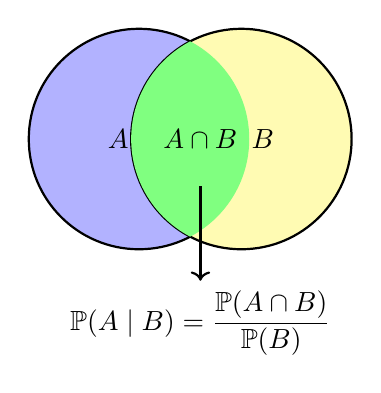
\begin{tikzpicture}[scale=1]
    % Centers and radius
    \def\r{1.4}
    \coordinate (Acenter) at (0,0);
    \coordinate (Bcenter) at (1.3,0);

    % Draw sets A and B with blue and yellow fills
    \draw[thick, fill=blue!30] (Acenter) circle (\r) node[left] {$A$};
    \draw[thick, fill=yellow!30] (Bcenter) circle (\r) node[right] {$B$};

    % Shaded intersection: clip to B and fill A to get A \cap B colored green
    \begin{scope}
      \clip (Bcenter) circle (\r);
      \fill[green!50] (Acenter) circle (\r);
    \end{scope}

    % Labels
    \node at ($(Acenter)!.6!(Bcenter)$) {$A\cap B$};

    % Formula node and arrow
    \node[below] (frac) at ($(Acenter)!.6!(Bcenter)-(0,1.8)$) {\(\displaystyle \P(A\mid B)=\frac{\P(A\cap B)}{\P(B)}\)};
    \draw[->, thick] ($(Acenter)!.6!(Bcenter)-(0,0.6)$) -- (frac.north);
  \end{tikzpicture}

  \begin{exampleblock}{Visual takeaway}
    \small
    Conditioning on $B$ means we restrict attention to the region $B$ (the right circle) and ask what fraction
    of $B$ is occupied by $A\cap B$ (the shaded overlap). The conditional probability is that fraction:
    \[\P(A\mid B)=\dfrac{\P(A\cap B)}{\P(B)}.\]
  \end{exampleblock}
\end{frame}

\begin{frame}{Conditional probability — a hands-on example}
  \small
  \textbf{Setup (standard deck, 52 cards).} \\
  Let $A$ = “card is a King” and $B$ = “card is a face card".

  \medskip
  \textbf{Unconditional probabilities}
  \begin{itemize}
    \item $\displaystyle \mathbb{P}(A) = \frac{4}{52} = \frac{1}{13}$
    \item $\displaystyle \mathbb{P}(B) = \frac{12}{52} = \frac{3}{13}$
  \end{itemize}

  \medskip
  \textbf{Conditional probability (definition only)}
  \[
    \mathbb{P}(A \mid B) \;=\; \frac{\mathbb{P}(A \cap B)}{\mathbb{P}(B)}.
  \]
  Since $A \cap B$ = “King that is also a face card” has 4 outcomes,
  \[
    \mathbb{P}(A \cap B) = \frac{4}{52} = \frac{1}{13}
    \quad\Rightarrow\quad
    \mathbb{P}(A \mid B) = \frac{\,\tfrac{1}{13}\,}{\,\tfrac{3}{13}\,} = \frac{1}{3}.
  \]
\end{frame}

\begin{frame}{Conditional probability — a hands-on example}
  \begin{exampleblock}{Intuition \& takeaway}
    \begin{itemize}
      \item The event $B$ ("card is a face card") restricts the sample space to 12 cards: $\{J, Q, K\}\times\{\heartsuit, \diamondsuit, \clubsuit, \spadesuit\}$.
      \item Within this restricted space, there are 4 Kings, so $\mathbb{P}(A \mid B) = 4/12 = 1/3$.
      \item This shows how conditioning on an event can significantly change the probability of another event.
    \end{itemize}

  \end{exampleblock}
\end{frame}

% Bayes Theorem
\begin{frame}{Bayes Theorem}
  \begin{block}{Bayes Theorem}
    Let \( A \) and \( B \) be two events, with \( \P(B) > 0 \). Then:
    \[
      \P(A\mid B) = \frac{\P(B\mid A) \, \P(A)}{\P(B)}.
    \]
  \end{block}

  \begin{itemize}
      \small
    \item \( \P(A\mid B) \): The probability of \( A \) given \( B \) (posterior).
    \item \( \P(B\mid A) \): The probability of \( B \) given \( A \) (likelihood).
    \item \( \P(A) \): The prior probability of \( A \).
    \item \( \P(B) \): The total probability of \( B \).
  \end{itemize}
  \begin{exampleblock}{Takeaway}
    \small
    \begin{itemize}
      \item \textbf{Bayes Theorem} is a fundamental theorem in probability that allows us to update the probability of a hypothesis based on new evidence.
      \item It expresses how the probability of an event \( A \), given another event \( B \), is related to the reverse conditional probability \( \P(B\mid A) \).
    \end{itemize}
  \end{exampleblock}
\end{frame}

\begin{frame}{Example — Dice}
  \begin{exampleblock}{Compute $\P(A\mid B)$ for the two-dice example}
    \small
    Recall: $A$ = "sum is 7", $B$ = "first die is even" with
    $\P(A)=6/36$, $\P(B)=18/36$, and $\P(A\cap B)=3/36$.

    Direct conditional formula:
    \[
      \P(A\mid B)=\frac{\P(A\cap B)}{\P(B)}=\frac{3/36}{18/36}=\frac{3}{18}=\frac{1}{6}.
    \]

    Using Bayes' theorem (alternative view):
    \[
      \P(B\mid A)=\frac{\P(A\cap B)}{\P(A)}=\frac{3/36}{6/36}=\frac{1}{2},
    \]
    hence
    \[
      \P(A\mid B)=\frac{\P(B\mid A)\,\P(A)}{\P(B)}=\frac{\tfrac{1}{2}\cdot\tfrac{1}{6}}{\tfrac{1}{2}}=\tfrac{1}{6}.
    \]
  \end{exampleblock}
\end{frame}

% Slide 6: Example of Bayes Theorem
\begin{frame}{Example — Medical diagnosis}
  \begin{exampleblock}{Compute $\P(\text{Disease}\mid\text{Positive})$}
    \small
    Assume: $\P(\text{Disease})=0.001$, $\P(+\mid\text{Disease})=0.99$, and $\P(+\mid\text{No Disease})=0.01$.

    First compute the marginal probability of a positive test (law of total probability):
    \[
      \P(+) = \P(+\mid\text{Disease})\P(\text{Disease}) + \P(+\mid\text{No Disease})\P(\text{No Disease})
    \]
    Numerically:
    \[
      \P(+) = 0.99\times0.001 + 0.01\times0.999 = 0.00099 + 0.00999 = 0.01098.
    \]

    Now apply Bayes' theorem:
    \[
      \P(\text{Disease}\mid +) = \frac{\P(+\mid\text{Disease})\,\P(\text{Disease})}{\P(+)} = \frac{0.99\times0.001}{0.01098} \approx 0.0902.
    \]
    So a positive test yields about a $9.02\%$ chance of actually having the disease.
  \end{exampleblock}
\end{frame}

\begin{frame}{Example — Medical diagnosis (negative test)}
  \begin{exampleblock}{Compute $\P(\text{Disease}\mid\text{Negative})$}
    \small
    Using the same assumptions as before: $\P(\text{Disease})=0.001$, $\P(+\mid\text{Disease})=0.99$, $\P(+\mid\text{No Disease})=0.01$. Thus $\P(-\mid\text{Disease})=0.01$ and $\P(-\mid\text{No Disease})=0.99$. Compute the marginal for a negative test:
    \[
      \P(-)=\P(-\mid\text{Disease})\P(\text{Disease})+\P(-\mid\text{No Disease})\P(\text{No Disease})
    \]
    Numerically:
    \[
      \P(-)=0.01\times0.001 + 0.99\times0.999 = 0.00001 + 0.98901 = 0.98902.
    \]

    Apply Bayes' theorem:
    \[
      \P(\text{Disease}\mid -)=\frac{\P(-\mid\text{Disease})\,\P(\text{Disease})}{\P(-)}=\frac{0.01\times0.001}{0.98902}\approx 1.011\times10^{-5}.
    \]
    This is about $0.00101\%$ (very small): a negative test makes the disease extremely unlikely.
  \end{exampleblock}
\end{frame}

% Section 3: Independence
\section{Independence}

% Slide 7: Independence Among Events
\begin{frame}{Independence Among Events}
  \small
  \begin{block}{Definition}
    Two events $A$ and $B$ are independent if the occurrence of one does not affect the probability of the other. Formally:
    \[
      \P(A \cap B) = \P(A)\,\P(B).
    \]
    Equivalently (when $\P(A),\P(B)>0$):
    \[
      \P(B\mid A) = \P(B) \quad\text{and}\quad \P(A\mid B) = \P(A).
    \]
  \end{block}

  \begin{exampleblock}{Takeaway}
    \begin{itemize}
      \item Independence means that knowing \( A \) occurred gives no information about whether \( B \) occurred, and vice versa.
      \item Independence simplifies computations: intersections factor into products.
      \item In practice, check independence via $\P(A\cap B)=\P(A)\P(B)$ or the conditional form.
    \end{itemize}
  \end{exampleblock}
\end{frame}

\begin{frame}{Independence Among Events \textemdash{} Visual}
  \centering
  % Venn-style diagram of events within a sample space rectangle
  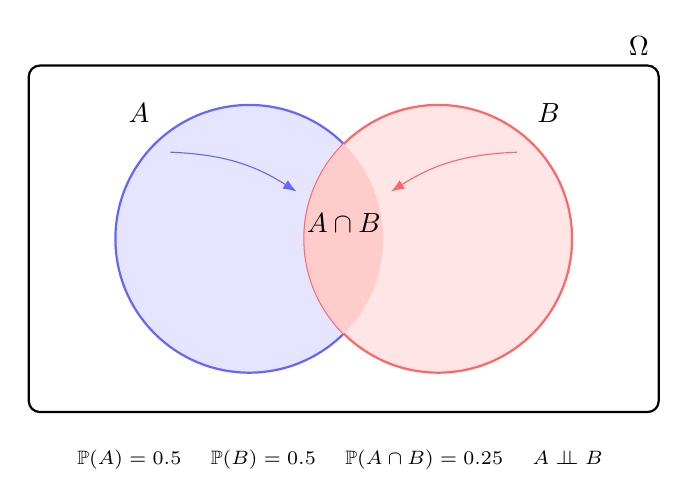
\begin{tikzpicture}[x=1cm,y=1cm]
    % Sample space rectangle
    \draw[rounded corners=4pt, thick] (-4,-2.2) rectangle (4,2.2);
    \node[anchor=south east] at (4,2.2) {$\Omega$};

    % Two events A and B (slightly smaller to create more whitespace)
    \def\eventrad{1.7}
    \filldraw[fill=blue!10, draw=blue!60, thick] (-1.2,0) circle (\eventrad);
    \filldraw[fill=red!10, draw=red!60, thick] (1.2,0) circle (\eventrad);

    % Intersection shading (A ∩ B)
    \begin{scope}
      \clip (-1.2,0) circle (\eventrad);
      \fill[red!20] (1.2,0) circle (\eventrad);
    \end{scope}

    % Labels
    \node at (-2.6,1.6) {$A$};
    \node at (2.6,1.6) {$B$};
    \node at (0,0.2) {$A\cap B$};

    % Example probabilities (illustrative) \textemdash{} lowered and smaller to avoid overlap
    \node[align=center, anchor=north, inner sep=2pt, fill=white, fill opacity=0.85, text opacity=1]
    at (0,-2.6) {\scriptsize
      $\P(A)=0.5\quad\ \P(B)=0.5\quad\ \P(A\cap B)=0.25\quad\ A\indep B$
    };

    % Decorative arrows to emphasize independence relation
    \draw[->, >=Latex, blue!60] (-2.2,1.1) to[bend left=15] (-0.6,0.6);
    \draw[->, >=Latex, red!60] (2.2,1.1) to[bend right=15] (0.6,0.6);
  \end{tikzpicture}

  \vspace{0.3em}
  {\small Visual intuition: events are subsets of $\Omega$; independence here matches $\P(A\cap B)=\P(A)\,\P(B)$.}
\end{frame}

% Example of Independence
\begin{frame}{Independence of Events — Coin Toss Example}
  \small
  \textbf{Experiment:} Toss two fair coins. \\[0.5em]

  \textbf{Sample space (equiprobable outcomes):}
  \[
    \{ HH, HT, TH, TT \}, \quad \mathbb{P}(\text{each}) = \tfrac{1}{4}.
  \]

  \medskip
  \textbf{Joint probability table:}

  \begin{center}
    \begin{tabular}{c|c|c|c}
      & Second = H & Second = T & Total \\
      \hline
      First = H & $1/4$ & $1/4$ & $1/2$ \\
      \hline
      First = T & $1/4$ & $1/4$ & $1/2$ \\
      \hline
      Total & $1/2$ & $1/2$ & $1$
    \end{tabular}
  \end{center}

  \medskip
  \textbf{Check independence:}
  \begin{itemize}
    \item $A =$ “First coin is Heads” $\;\Rightarrow\; \mathbb{P}(A)=1/2$.
    \item $B =$ “Second coin is Heads” $\;\Rightarrow\; \mathbb{P}(B)=1/2$.
    \item Joint: $\mathbb{P}(A \cap B) = 1/4 = (1/2)(1/2)$.
    \item $\Rightarrow$ $A$ and $B$ are \textbf{independent}.
  \end{itemize}
\end{frame}

\begin{frame}{Non-Independence of Events — Coin Toss Example}
  \small
  \textbf{Experiment:} Toss two fair coins. \\[0.5em]

  \textbf{Sample space (equiprobable outcomes):}
  \[
    \{ HH, HT, TH, TT \}, \quad \mathbb{P}(\text{each}) = \tfrac{1}{4}.
  \]

  \medskip
  \textbf{Joint probability table:}

  \begin{center}
    \begin{tabular}{c|c|c|c}
      & At least one Head & No Head (TT) & Total \\
      \hline
      First = H & $1/2$ & $0$   & $1/2$ \\
      \hline
      First = T & $1/4$ & $1/4$ & $1/2$ \\
      \hline
      Total & $3/4$ & $1/4$ & $1$
    \end{tabular}
  \end{center}

  \medskip
  \textbf{Check independence:}
  \begin{itemize}
    \item $A =$ “First coin is Heads” $\;\Rightarrow\; \mathbb{P}(A)=1/2$.
    \item $D =$ “At least one Head” $\;\Rightarrow\; \mathbb{P}(D)=3/4$.
    \item Joint: $\mathbb{P}(A \cap D) = 1/2$.
    \item Product: $\mathbb{P}(A)\,\mathbb{P}(D) = (1/2)(3/4) = 3/8$.
    \item Since $1/2 \neq 3/8$, $A$ and $D$ are \textbf{not independent}.
  \end{itemize}
\end{frame}

\begin{frame}{Mutual Independence — Definition and Intuition}
  \small
  \begin{block}{Definition}
    \textbf{Formal definition (arbitrary family):}
    Let $\{A_i\}_{i\in I}$ be a (possibly infinite) family of events on $(\Omega,\mathcal{F},\mathbb{P})$.
    We say $\{A_i\}_{i\in I}$ is \textbf{mutually independent} if for every finite, nonempty subset
    $J \subseteq I$ with $|J|\ge 2$,
    \[
      \mathbb{P}\!\Bigl(\bigcap_{j\in J} A_j\Bigr)
      \;=\; \mathbb{P}\bigl( A_{i_1} \cap \cdots \cap A_{i_k} \bigr) \;=\; \mathbb{P}(A_{i_1}) \cdots \mathbb{P}(A_{i_k}) \;=\; \prod_{j\in J}\mathbb{P}(A_j).
    \]
  \end{block}

  \emph{Equivalently: all finite subcollections are independent (the product rule holds for every finite intersection).}

  \medskip
  \begin{itemize}
    \item No matter which \emph{finite} subset of events you look at, knowing some of them occurred does not change the probability of any combination of the others.
    \item This is stronger than pairwise independence: it requires factorization for all $k$-way intersections ($k=2,3,\dots$) drawn from the family.
    \item For infinite families, mutual independence is still checked via \emph{all finite} subfamilies (not an infinite intersection).
  \end{itemize}
\end{frame}

\begin{frame}{Pairwise vs. Mutual Independence}
  \textbf{Independence of two events:}
  \[
    A, B \text{ independent} \quad \iff \quad \mathbb{P}(A \cap B) = \mathbb{P}(A)\,\mathbb{P}(B).
  \]

  \textbf{Pairwise independence of a family:}
  \begin{itemize}
    \item Every \emph{pair} $(A_i, A_j)$ is independent.
    \item Only checks 2-event intersections.
  \end{itemize}

  \medskip
  \textbf{Mutual independence of a family:}
  \begin{itemize}
    \item Stronger condition: independence holds for \emph{every sub-collection}, not only pairs.
    \item Requires all $k$-way intersections to factorize, for all $k=2,3,\dots,n$.
  \end{itemize}

  \begin{exampleblock}{Key takeaway}
    Pairwise independence does \emph{not} imply mutual independence.
  \end{exampleblock}
\end{frame}

\begin{frame}{Example — Pairwise but not Mutual Independence}
  \small
  \textbf{Experiment:} Toss two fair coins.

  \begin{itemize}
    \item $A =$ “First coin is Heads”.
    \item $B =$ “Second coin is Heads”.
    \item $C =$ “The two coins show the same result”.
  \end{itemize}

  \textbf{Check pairwise independence:}
  \begin{itemize}
    \item $\mathbb{P}(A)=\mathbb{P}(B)=\tfrac{1}{2}, \quad \mathbb{P}(C)=\tfrac{1}{2}$.
    \item $\mathbb{P}(A \cap B)=\tfrac{1}{4} = \mathbb{P}(A)\mathbb{P}(B)$.
    \item $\mathbb{P}(A \cap C)=\tfrac{1}{4} = \mathbb{P}(A)\mathbb{P}(C)$.
    \item $\mathbb{P}(B \cap C)=\tfrac{1}{4} = \mathbb{P}(B)\mathbb{P}(C)$.
    \item $\Rightarrow$ $A, B, C$ are pairwise independent.
  \end{itemize}

  \textbf{But not mutually independent:}
  \[
    \mathbb{P}(A \cap B \cap C) = \tfrac{1}{4}
    \quad \neq \quad
    \mathbb{P}(A)\,\mathbb{P}(B)\,\mathbb{P}(C) = \tfrac{1}{8}.
  \]
\end{frame}

% Slide 9: Summary
\begin{frame}{Summary}
  \begin{exampleblock}{What we covered}
    This lesson introduced the foundational concepts of probability theory that underpin statistical analysis.
    \bigskip

    \begin{itemize}
      \item We motivated the study of statistics and its applications.
        \medskip
      \item We introduced event spaces, events, and their realizations.
        \medskip
      \item We discussed how to define and manipulate probabilities on sets.
        \medskip
      \item We introduced Bayes theorem, which allows us to update probabilities with new information.
        \medskip
      \item We explained the concept of independence between events.
    \end{itemize}

  \end{exampleblock}
\end{frame}

% References
\begin{frame}{References}
  \begin{itemize}
    \item Textbook: "Introduction to Probability and Statistics" by Mendenhall, Beaver, and Beaver.
    \item Online resources: \url{https://www.khanacademy.org/math/statistics-probability}
  \end{itemize}
\end{frame}

% End document
\end{document}
